\documentclass[12pt,letterpaper]{report}
\usepackage[square,numbers]{natbib}
\usepackage{geometry}
\usepackage{fancyhdr}
\usepackage{afterpage}
\usepackage{graphicx}
\usepackage{amsmath,amssymb,amsbsy}
\usepackage{dcolumn,array}
\usepackage{tocloft}

% for title case
\usepackage{titlecaps}
\Addlcwords{and, the, or, of, that, our, by, a, prevent, for}

% avoid widows
\usepackage[all]{nowidow}
\clubpenalty=10000

\usepackage{asudis}
%% These are for including code
%% and for upquotes
\usepackage[T1]{fontenc}
\usepackage{textcomp}
\usepackage{listings}
\usepackage{listingsutf8}
\usepackage{comment}
\usepackage{color}
%\usepackage{dirtytalk} % for quotations
\usepackage[justification=centering]{caption}
\usepackage[pageanchor=true,plainpages=false,pdfpagelabels,bookmarks,bookmarksnumbered,hidelinks]{hyperref}


% for footnotes in tables
\usepackage{tablefootnote}

% for arithmetic
\usepackage{xintexpr}

\usepackage{textcomp}     % access \textquotesingle

\definecolor{mygray}{rgb}{0.6,0.6,0.6}
\definecolor{lightgray}{rgb}{0.92,0.92,0.92}
\definecolor{darkgreen}{rgb}{0,0.7,0}
% default options for listings
\lstset{
	backgroundcolor=\color{lightgray},
	basicstyle=\footnotesize,
	breaklines=true, 
	captionpos=b,
	commentstyle=\color{darkgreen}, 
	frame=single,
	keywordstyle=\color{blue}, 
	numbers=left,
	numbersep=5pt,
	numberstyle=\tiny\color{mygray},
	rulecolor=\color{black},
	showstringspaces=false,
	upquote=true
}

	
\newcommand{\dq}[1]{``{#1}''}
%% THIS IS THE DATA FOR OUR THESIS, UPDATING HERE WILL UPDATE EVERYWHERE %%
\newcommand{\urls}{21,675,680\xspace}

\newcommand{\forms}{6,794,917\xspace}
\newcommand{\formsDelta}{31.35\%\xspace}

\newcommand{\emailforms}{1,132,157\xspace}
\newcommand{\emailformsDelta}{16.66\%\xspace}

\newcommand{\fuzzed}{934,016\xspace}
\newcommand{\fuzzedDelta}{82.50\%\xspace}

\newcommand{\recd}{52,724\xspace}
\newcommand{\recdDelta}{5.64\%\xspace}

\newcommand{\malfuzzed}{46,156\xspace}
\newcommand{\malfuzzedDelta}{87.54\%\xspace}

\newcommand{\success}{673\xspace}
\newcommand{\successDelta}{1.46\%\xspace}
\newcommand{\successWebsitesDelta}{0.029\%\xspace} % calc 296/1,019,921

\newcommand{\domains}{296\xspace}
\newcommand{\emailedDefaultmailbox}{111\xspace}
\newcommand{\responses}{15\xspace}
\newcommand{\confirmed}{10\xspace}
\newcommand{\ips}{413\xspace}

\newcommand{\ipsblacklist}{106\xspace}
\newcommand{\ipsblacklistmulti}{33\xspace}

\newcommand{\ehibcc}{329\xspace}
\newcommand{\ehixcheck}{396\xspace}
\newcommand{\ehito}{163\xspace}
\newcommand{\ehibccxcheck}{216\xspace}
\newcommand{\ehitoxcheck}{13\xspace}
\newcommand{\ehinuserxcheck}{219\xspace}
\newcommand{\ehiuniquenuserxcheck}{181\xspace}

% these refer to unique domains, not unique forms
\newcommand{\uniqueforms}{1,019,921\xspace}
\newcommand{\uniqueemailforms}{197,570\xspace}

\newcommand{\ehi}{E-\nobreak{}mail Header Injection\xspace}

\begin{document}
%-----------------------front matter
\pagenumbering{roman}
\title{iGen: Toward Automatic Generation and\\
 Analysis of Indicators of Compromise (IOCs)\\
 using Convolutional Neural Network}
\author{Anupam Panwar}
\degreeName{Master of Science}
\paperType{Thesis}
\defensemonth{April}
\defenseyear{2017}
\gradmonth{May}
\gradyear{2017}
\chair{Gail-Joon Ahn}
\memberOne{Adam Doup\'e}
\memberTwo{Ziming Zhao}
\maketitle
\doublespace
\begin{abstract}

Field of cyber threats is evolving rapidly and every day multitude of new information
about malwares and Advanced Persistent Threats (APTs) is generated by the
security professionals in the form of malware reports, blog articles, forum posts etc.
However, currently data received from different sources is examined and interpreted
by an analyst manually, a procedure that extremely obscures the practical use of this
data in an enterprise’s security infrastructure. Most of traditional approaches just
consider either one or two data sources for the generation of Indicators of Compromise
(IOCs) and misses some of the most valuable IOCs from other data sources.
This leaves some scope for attackers to bypass the defense systems. Additionally, current state of art lacks support to diverse IOC formats (e.g. STIX, OpenIOC, snort
etc.) which further reduce the effectiveness of these tools. Most importantly, lots
of Threat Intelligence (TI) tools are generating IOCs directly using regex expression
without understanding the contextual meaning of those IOCs from the data sources
which allows the tools to include lot of false positives during the process of IOCs
creation.

To overcome these limitations, we propose iGen, a novel approach to fully automate
the process of IOC generation and analysis. iGen consists of different modules like data acquisition module, malware analysis module, intelligent IOC extraction module and security rule generator module. All these modules are arranged in a work-flow to fully automate the IOC generation process.  Proposed approach is based on
the idea that our model can understand English texts like human beings, and extract
the IOCs from the different data sources intelligently. Identification of the IOCs
is done on the basis of the syntax and semantics of the sentence as well as context
words (e.g., “attacked”, “suspicious”) present in the sentence which helps the approach
work on any kind of data source. Our proposed technique, first removes the
words with no contextual meaning like stop words and punctuations etc. Then using
the rest of the words in the sentence and output label (IOC or non-IOC sentence), our model intelligently learn to classify sentences into IOC and non-IOC sentences.
Once IOC sentences are identified using this Convolutional Neural Network (CNN)
based approach, next step is to identify the IOC tokens (like domains, IP, URL) in
the sentences. This CNN based classification model helps in removing false positives
(like IPs which are not malicious). Afterwards, IOCs extracted from different data
sources are correlated to find the links between thousands of apparently unrelated
attack instances, particularly infrastructures shared between them. Our approach
fully automates the process of IOC generation from gathering data from different
sources to creating rules (e.g. OpenIOC, snort rules, STIX rules) for deployment on
the security infrastructure.
\end{abstract}

\dedicationpage{To my loving family and friends for their patience and support. I want to give special
note of appreciation to my late mother Madhu Panwar for her sacrifice and hard work which she
put in to teach me the importance of hardwork and being good human. She always wanted to see
me succeed. She sacrificed a lot of her personal interest and ambitions to provide all the necessary
resources needed for my success. Mom, this is for you! My twin brother Anurag motivated me to
do research and taught me never give up attitude. My father Dr. H R Panwar always supported
my decision. My elder brother Anshuman worked as catalyst for my success. Finally, I am forever
indebted to my family for their understanding, endless patience and encouragement when it was
most required.}
\begin{center}
ACKNOWLEDGMENTS
\end{center}
My journey through my Computer Science degree both B.S and M.S has been an exciting one which has played a major role in my career and life, especially in enhancing my knowledge and experience in this field of study. Having had the opportunity to work with Dr.\ Gail-Joon Ahn for two years has been an insightful experience, and I am utmost grateful to him for having given me the opportunity to work on cutting edge research projects at the laboratory for Security Engineering for Future Computing (SEFCOM). Dr.\ Ahn has been a constant source of motivation through my graduate career at Arizona State University, and has contributed significantly towards my abilities in  reasoning, approaching and solving research problems impacting the society as a whole. I would like to extend my sincere gratitude to Dr.\ Partha Dasgupta  and Dr.\ Adam Doup\'e for serving on my committee and providing their valuable feedback on my thesis. 

My experience at the SEFCOM lab has provided me with great opportunities in my professional career, and has enabled me to connect with brilliant and innovative individuals who have always been there to provide valuable inputs during my research work. I would specially like to express my gratitude to Marthony Taguinod, who worked with me in the development of our test-bed for Cisco Inc. In addition to my committee and the SEFCOM lab members, I would also like to thank Cisco Inc.\ and more specifically Dr.\ Rodolfo Milito, for their support in the Fog Computing project and their valuable input during the development of our test-bed. Finally, and most importantly, I would like to extend my sincere love and regards to my parents for being a constant source of motivation and support throughout my academic career.
\tableofcontents
% This puts the word "Page" right justified above everything else.
\addtocontents{toc}{~\hfill Page\par}
% Asking LaTeX for a new page here guarantees that the LOF is on a separate page
% after the TOC ends.
\newpage
% Making the LOT and LOF "parts" rather than chapters gets them indented at
% level -1 according to the chart: top of page 4 of the document at
% ftp://tug.ctan.org/pub/tex-archive/macros/latex/contrib/tocloft/tocloft.pdf
\addcontentsline{toc}{part}{LIST OF TABLES}
\renewcommand{\cftlabel}{Table}
\listoftables
% This gets the headers for the LOT right on the first page.  Subsequent pages
% are handled by the fancyhdr code in the asudis.sty file.
\addtocontents{lot}{Table~\hfill Page \par}
\newpage
\addcontentsline{toc}{part}{LIST OF FIGURES}
\addtocontents{lof}{Figure~\hfill Page \par}
\addtocontents{toc}{CHAPTER \par}
\renewcommand{\cftlabel}{Figure}
\listoffigures
% This gets the headers for the LOF right on the first page.  Subsequent pages
% are handled by the fancyhdr code in the asudis.sty file.
%----- XML Listing Configurations -------------
\definecolor{lightgray}{rgb}{.9,.9,.9}
\definecolor{darkgray}{rgb}{.4,.4,.4}
\definecolor{forestGreen}{RGB}{34,139,34}
\definecolor{orangeRed}{RGB}{255,69,0}
\definecolor{white}{RGB}{255,255,255}
 
\lstdefinelanguage{bpel}{
morekeywords={name,linkName,isolated,parallel,partnerLink,operation,portType,inputVariable,createInstance,
variable,element,location,importType,partnerLinkType,myRole,messageType,properties,level,outputVariable,
xmlns,version,encoding}
}
\lstdefinelanguage{xaml}{
morekeywords={TypeArguments,Name,Default,DisplayName,OperationName,ServiceContractName,Key,AddressUri,
CanCreateInstance, LogName, Message, MessageNumber, Expression,CorrelationHandle,Request}
}
 
\lstdefinelanguage{xml}{
        basicstyle=\small,
        sensitive=false,
}
 
\lstdefinestyle{workflowStyle}{
language=XML,
alsolanguage=bpel,
alsolanguage=xaml,
%Formatting
basicstyle=\scriptsize,
sensitive=true,
showstringspaces=false,
numbers=left,
numberstyle=\tiny,
tabsize=4,
numbersep=3pt,
extendedchars=true,
xleftmargin=2em,
lineskip=1pt,
breaklines,
captionpos=t,
%Coloring
backgroundcolor=\color{white},
morekeywords={BooleanExpression},
alsoletter={:,<,>,/,?},
morestring=[b]{"},
morecomment=[s]{<!--}{-->},keywordstyle=\color{forestGreen},
identifierstyle=\color{blue}\ttfamily,
stringstyle=\color{orangeRed}\ttfamily,
commentstyle=\color{forestGreen}\ttfamily
}
 
 
\lstnewenvironment{workflow-code}[2]{
\lstset{caption=#1,label=#2,style=workflowStyle}
}{}
%-----------------------body
\doublespace
\pagenumbering{arabic}
\chapter{INTRODUCTION}
\label{chap:introduction}
According to Verizon's 2016 Data Breach Investigations Report~\cite{verizon}, over 100,000 security incidents were reported in 2016 across 82 countries, which is a 25\% increase over the prior year. Because the number of security threats and breaches is rapidly increasing over time, every organization is attempting to protect their systems and their data. The threat landscape is always progressing, and the information security risk is increasing because of the organization's dependence on computing systems. This constantly shifting and constantly increasing number of threats results in tremendous pressure on organizations to manage threats.
% Adam: I don't understand what the next two sentences are trying to say. Could they be reworded?
Though abundant information is available in the form of unstructured data, it is very difficult and time-consuming to mine meaningful information based on which preemptive measures can be established. This attracts more and more researchers towards Threat Intelligence (TI) as it helps to understand threats using the deluge of data and provides actionable insights.

Threat intelligence (TI) is proof-based knowledge, which includes reasoning, context, mechanism, indicators, implications, and actionable advice, about an existing or evolving cyber-attack that can be used to create preventive measures in advance~\cite{rob}.  Attackers consistently exploit systems and networks to steal sensitive information, to take control of the target system, or for ransom (using ransomware)~\cite{gorman}. TI allows an organization to expand its visibility into the fast-growing threat landscape, can allow early identification of an attack, and successfully prevent the attack. 

Indicators of Compromise (IOCs) are forensic artifacts that are used as signs that a system has been compromised by an attacker or that a system has been infected with a particular piece of malware~\cite{catakoglu}. The intent of accumulating IOCs related to malware or an attack is to be able to state, with a relatively high degree of confidence, whether or not such artifacts are present in a given environment. The goal of TI is to help security professional provide data-backed reasoning of why an artifact is identified as an IOC or not. Concretely, IOCs are composed of some combination of IP addresses, hostnames, filenames, processes, services, Windows registry entries, or hashes~\cite{andress}.

Figure~\ref{fig:ioc} explains the typical life cycle for the use of IOCs in an organization. This life cycle consists of five steps: data collection, data analysis, IOC creation, deployment of IOCs on security infrastructure, and identification of affected systems using deployed IOCs. As a final step, log data of these compromised systems is collected and used for the creation new IOCs, which feeds back into the IOC life cycle in a cyclical way.

Several standards are commonly used to represent IOCs for expressing cyber-threat intelligence information such as: OpenIOC~\cite{openioc}, Structured Threat Information eXpression (STIX)~\cite{stix}, Cyber Observable eXpression (CybOX)~\cite{cybox}, Trusted Automated eXchange of Indicator Information (TAXII)~\cite{taxii}, Snort~\cite{snort}, Suricata~\cite{suricata}, YARA~\cite{yara}, Malware Attribute Enumeration and Characterization (MAEC)~\cite{maec}, and Common Attack Pattern Enumeration and Classification (CAPEC)~\cite{capec}.

IOCs can help an organizations' security personnel to attain full automation: Given a set of IOCs for a particular security event, security tools scan through an environment or infrastructure to identify the existence of any IOC on the systems in question. IOCs complement and augment existing solutions, such as Intrusion Detection Systems (IDS) or Security Information and Event Managements (SIEMs), by providing an additional and important set of information that can be used to decide whether a particular artifact being examined is malicious or not. IOCs provide a rapid route to detect new or zero-day attacks for which virus signatures or detection rules have yet to be developed for existing security tools. Thus, timely generation of IOCs is important. Also, IOC formats document a threat in a consistent fashion, thus it becomes easier for organizations to share this threat information. 

However, effective collection and sharing of threat information is a challenge. Current threat intelligence systems have following limitations: 
\begin{itemize}
 \item[$\bullet$ ] Threat data received from different sources, such as malware reports, APT white-papers, etc., is examined and interpreted
by security analysts \emph{manually}, a procedure that is timely and error-prone, which limits the practical usefulness of this
data in an organizations' security infrastructure. 
  \item[$\bullet$ ] Most of the traditional approaches consider either one or two data sources for the generation of Indicators of Compromises
(IOCs) and miss valuable IOCs from alternative data sources, such as blog articles about recent attacks.
  \item[$\bullet$ ] Current state-of-the-art lacks support of diverse IOC formats (e.g., STIX, OpenIOC, or snort) which further reduces the effectiveness of these tools. 
\item[$\bullet$ ] Most importantly, many TI tools generate IOCs directly using regular expressions and white-listings from security literature or blog articles~\cite{otx} without understanding the contextual meaning of those IOCs from the data sources which allows the tools to include lot of false positives during the process of IOCs creation.
\end{itemize}

%iGen is tackling all these limitation by intelligently collecting and exchanging the information in the form of IOCs (e.g. virus signatures, IPs, domains, MD5 hashes etc.). After the collection, iGen automatically transforms these IOCs into different threat information sharing standards such as STIX , OpenIOC , and Snort rules etc. and fed into different defense mechanisms (e.g. Intrusion Detection Systems (IDS) etc). Biggest challenge in the field of TI is to intelligently gather such information from large amount of data and timely deploy it on defense mechanisms.

In this project we present iGen, which is a system that tackles all of these limitation by intelligently collecting threat information from publicly available security resources and sharing the threat information in the form of IOCs (e.g., virus signatures, IPs, domains, or MD5 hashes). iGen automates the entire process of collecting publicly available data (data collection) to IOC generation. iGen supports a flexible system to collect data from diverse data sources. Currently, iGen collects data from 20 security blogs, an APT reports database~\cite{apt}, and a malware analysis system. The flexible nature of the system means that new data sources can be easily added. Note that the input to iGen is in unstructured English text, therefore iGen must understand the semantics of the sentences present in the input data to categorize IOC-alike strings into IOC or non-IOCs. Also, we added a practical improvement to iGen that allows transforming these IOCs into various threat information sharing standards.

% Adam: This is way too much detail for the intro
First module in iGen is data acquisition module which collects key observations from the data sources like APT reports, malware analysis reports and blog articles. This module collects these reports in real-time and keep iGen updated with new IOCs from recent malware and APTs. In parallel, malware analysis system looks for new malware on web and generate malware analysis report for those samples.   All the different kinds of reports accumulated from different data sources are then presented to machine learning based IOC extractor. IOC extractor module decides the parsing strategy based on the type of report. Since, malware analysis reports are based on real malware and available in machine readable format (e.g. JSON file). In this case, IOC extraction was done using a parser which accrue IOCs based on the JSON schema. But security reports or blog articles are relatively complex which tend to describe IOCs in intricate manner in English text using some context terms like ``download'', ``malware'' etc. Google's tensorflow~\cite{abadi} based Convolutional Neural Netowrk~\cite{krizhevsky} model was used to classification all the sentences in these reports into IOC or non-IOC sentences~\cite{bengio,yih,mikolov,collobert}. Once sentence classification is done, next step is to identify IOCs intelligently. More explicitly, after classifying the sentence in the article into IOC and non-IOC sentences. iGen utilizes a set of regular expressions (regex) to locate IOC tokens (e.g., IP, hostname, domain, md5 etc.) within the sentence. Then, iGen extract these IOC tokens and convert them to machine-readable formats (IOC formats) which can be used directly by security tools.

Simple extraction of IOCs from publicly available security resources is straightforward: regular expressions can extract MD5s, URLs, filenames, filepaths, etc. However, this na\"{\i}ve approach will result in a significant amount of false positives: these security resources will include MD5s, URLs, and filenames that are \emph{relevant to the security incident but are not malicious, and thus not an IOC}. Therefore, we need an approach that can automatically filter these potential IOCs \emph{based on the context}.
While prior work has shown that filtering potential IOCs can be done with manual creation of features~\cite{liao}, iGen leverages a deep-learning Convolutional Neural Network, which selects features automatically. This enables iGen to be more effective and to use diverse data sets. 

The main contributions of this paper are the following:
\begin{itemize}
 \item[$\bullet$ ] We present the design of a novel system for intelligently generating IOCs, with high confidence, from different data sources using Convolutional Neural Networks (CNNs) (Section 3). 
  \item[$\bullet$ ] A prototype implementation of our design in a tool called iGen (Section 4).
  \item[$\bullet$ ] An evaluation of iGen with other state-of-the-art methods. iGen identified around 400,000 IOCs with a precision and recall of 95\% and 99\% respectively (Section 5). 
\end{itemize}

\chapter{BACKGROUND} \label{chap:background}
In this section, we provide the background necessary for understanding the design of iGen. In Section~\ref{ti}, we describe Threat intelligence and how it is consumed by security tools. Then, in Section~\ref{cnn}, we describe Convolutional Neural Network (CNN) and how it can be used in iGen.  

\section{Threat Intelligence} \label{ti}

Given the increasing number and rapidly evolving nature of current threats, quick sharing and exchange of relevant threat information is the key to swiftly detecting, understanding, and responding to cyber-attacks. Threat intelligence is two things: (1) a process of collection of knowledge that defines security threats, which empowers an organization to determine its responses at the strategic, operational, and tactical levels, and (2) information that has been analyzed to discover actionable insights. Actionable threat intelligence is insight that an organization can act on—--it enables informed decision-making that results in improved outcomes. 

Threat intelligence consists of two words: ``Threat'' and ``Intelligence''. ``Threat'' is an agent (that is, a menace or hazard) that takes advantage of the vulnerability. Whereas, ``Intelligence'' can be defined as: 
\begin{itemize}
 \item[$\bullet$ ] Act of generating new information by correlating information from different sources.
  \item[$\bullet$ ] Capacity to know or understand.
  \item[$\bullet$ ] Knowledge imparted through study, research or experience.
\end{itemize}


\subsection{Consumption of Threat Intelligence}

Indicators of Compromise (IOCs) are used for organizations to exchange threat intelligence. There are different standards for IOCs which includes OpenIOC, STIX, and snort rules. OpenIOC was introduced by Mandiant in 2011.  It is primarily used in Mandiant products, but has also been released as an open standard. OpenIOC provides definitions for specific technical details including over 500 indicator terms. Adding new terms is easy because the terms are separated from the main schema. Most of the terms are host-centric.

Similarly, STIX is another format for storing IOCs. STIX allows defining threat information, including threat details, as well as the \emph{context} of the threat. STIX is developed by Mitre, and is designed to support four cyber threat use cases: investigating cyber threats, stating indicator patterns, response activities management, and sharing threat information. STIX uses XML to define threat-related constructs such as exploit target, campaign, indicator, threat actor, and TTP.

Snort is an open-source network intrusion prevention system (IPS)~\cite{sekar}, which  executes real-time traffic analysis and packet-logging on IP networks. It is also capable of performing protocol analysis, content searching, and matching, and can be used to detect a variety of attacks and probes, such as buffer overflows, stealth port scans, CGI attacks, SMB probes, OS fingerprinting attempts, and more. Snort uses a rule language to describe traffic that it should collect or pass, as well as a detection engine that uses a modular plug-in architecture. Rules created using this language are called snort rules.

Suricata rules are the defacto method for sharing and matching threat intelligence against network traffic. A suricata rule has three components: The action, header and rule-options.
%Adam: The above paragraph needs more information

%iGen has capabilities to transform IOCs related to particular event or incident into different output formats mentioned above.  These output formats can be directly consumed by different security mechanisms like IDS, IPS etc. This helps iGen further reduce the manual task of converting the IOCs into different rules/formats. 

\section{Convolutional Neural Network Architecture} \label{cnn}

Recently, different models based on deep learning have achieved significant results in computer vision and speech recognition. Convolutional Neural Networks (CNNs) were responsible for major breakthroughs in image classification~\cite{krizhevsky} and are the core of most computer vision systems today, from Facebook's automated photo tagging~\cite{stone} to self-driving cars~\cite{bojarski}. 

In the case of Natural Language Processing (NLP), much of the work that uses deep learning methods involves learning word vector representations through neural language models and performing composition over the learned word vectors for classification tasks. Word vectors, wherein words are projected from a sparse, 1-of-$V$ encoding (here $V$ is the vocabulary size) onto a lower dimensional vector space via a hidden layer, are essentially feature extractors that encode semantic features of words in their dimensions. In such compact representations, semantically close words are likewise close--in euclidean or cosine distance---in the lower dimensional vector space~\cite{mikolov}.

Recently, researchers have also started applying CNNs with word embeddings to problems in Natural Language Processing (NLP) and got some interesting results. CNNs utilize layers with convolving filters that are applied to local features. CNNs are effective for NLP and have achieved excellent results in semantic parsing, search query retrieval, sentence modeling, and other traditional NLP tasks.

\subsection{Convolution}
%
%\begin{figure}
%  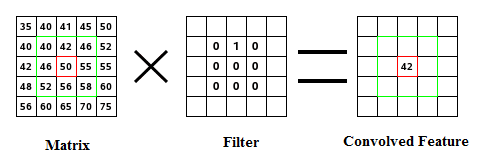
\includegraphics[width=\linewidth]{convolution.jpg}
%  \caption{Convolution with 3x3 filter.}
%  \label{fig:lifecycle}
%\end{figure}

%Convolution is a sliding window function applied to a matrix. As shown in figure 2, matrix on the left represents a black and white image. Each entry in the matrix corresponds to one pixel, 0 for black and 1 for white. The sliding window is called a kernel, filter, or feature detector. Here we use a $3\times3$ filter, multiply its values element-wise with the original matrix, then sum them up. To get the full convolution we do this for each element by sliding the filter over the whole matrix. Final matrix created after applying the filter is called convolved feature. 

Convolution~\cite{hu} is a sliding window function applied to a matrix. The sliding window is called a kernel, filter, or feature detector. Here we use a $N\times N$ filter, multiply its values element-wise with the original matrix, then sum them. To get the full convolution we do this for each element by sliding the filter over the whole matrix. Final matrix created after applying the filter is called convolved feature. 


\subsection{Convolution Neural Network}
CNNs are fundamentally several layers of convolutions with nonlinear activation functions like rectified linear unit (ReLU)~\cite{nair} or hyperbolic tangent (tanh)~\cite{goodfellow} applied to the results. In a traditional feedforward neural network, each input neuron to each output neuron in the next layer. It is called as fully connected layer, or affine layer. But it's different in case of CNNs. CNNs use convolutions over the input layer to compute the output. This results in local connections, where each region of the input is connected to a neuron in the output. Each convolution layer applies different filters, characteristically hundreds or thousands, and combines their results. Then pooling is performed using the pooling (subsampling) layer. We will discuss more in Chapter 4. CNN automatically learns the values of its filters based on the task during the training phase. For example, in image classification a CNN learns to detect edges from raw pixels in the first layer, then uses the edges to detect simple shapes in the second layer, and then uses these shapes to deter higher-level features, such as facial shapes in higher layers. The last layer is then a classifier that uses these high-level features. 



In the case of iGen, input to a CNN is sentences extracted from blog articles and security reports instead of image pixels. Each sentence is represented as a matrix. Each row vector of the matrix corresponds to one token, typically a word. That is, each row is vector that represents a word. These vectors might be, e.g., outputs from trained word2vec or GloVe~\cite{pennington} models. We will discuss more about the iGen CNN in Section 3.2. 



%CNNs are fundamentally several layers of convolutions with nonlinear activation functions like rectified linear unit (ReLU) or hyperbolic tangent (tanh) applied to the results. In a traditional feedforward neural network, each input neuron to each output neuron in the next layer. It is called as fully connected layer, or affine layer. But it’s different in case of CNNs. CNNs use convolutions over the input layer to compute the output. This results in local connections, where each region of the input is connected to a neuron in the output. Each convolution layer applies different filters, characteristically hundreds or thousands like the ones showed above in figure 2, and combines their results. Then pooling is performed using the pooling (subsampling) layer, we will talk more about it in section 3. CNN automatically learns the values of its filters based on the task during the training phase. For example, in Image Classification a CNN learn to detect edges from raw pixels in the first layer, then use the edges to detect simple shapes in the second layer, and then use these shapes to deter higher-level features, such as facial shapes in higher layers. The last layer is then a classifier that uses these high-level features. . A simple CNN is shown in the figure 3. 
%
%
%\begin{figure}
%  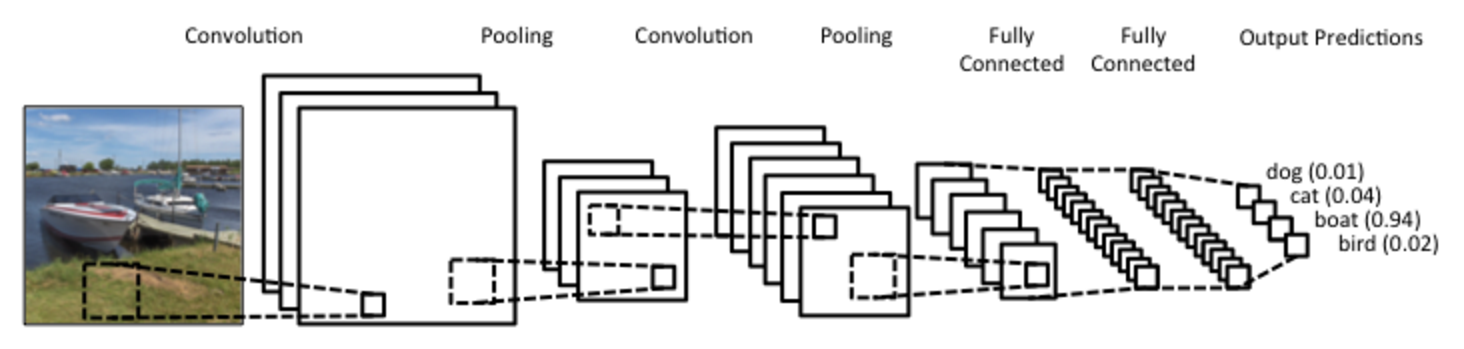
\includegraphics[width=\linewidth]{CNN.jpg}
%  \caption{Convolutional Neural Network (CNN) applied on an image.}
%  \label{fig:cnn}
%\end{figure}
%
%In case of iGen, input to CNN is sentences extracted from blog articles and security reports instead of image pixels. Each sentence is represented as a matrix. Each row vector of the matrix corresponds to one token, typically a word. That is, each row is vector that represents a word. These vectors might be, e.g., outputs from trained word2vec [] or GloVe [] models. We denote the dimensionality of the word vectors by $d$. If the length of a given sentence is $l$, then the dimensionality of the sentence matrix is $l \times d$. Here, sentences matrix can be effectively treated as an ‘image’, and perform convolution on it via linear filters. In text applications there is inherent sequential structure to the data. Because rows represent discrete symbols (namely, words), it is reasonable to use filters with widths equal to the dimensionality of the word vectors (i.e., $d$). Hence we can merely vary the ‘height’ of the filter, i.e., the number of adjacent rows considered jointly. We will refer to the height of the filter as the \emph{region size} of the filter [Collobert and Weston (2008)].
%
%Assume that a filter represented by the weight matrix $\mathbf{w}$ with region size $h$; $\mathbf{w}$ will contain $h \cdot d$ parameters to be estimated. Sentence matrix can be denoted by $\mathbf{S}\in \mathbb{R}^{l\times d}$ , and $\mathbf{S}[i:j]$ is used to represent the sub-matrix of  $\mathbf{S}$ from row $i$ to row $j$. The output sequence $\mathbf{out}\in\mathbb{R}^{l-h+1}$ of the convolution operator is obtained by repeatedly applying the filter on sub-matrices of $\mathbf{S}$:
%
%\begin{equation}
%out_i = \mathbf{w}\cdot \mathbf{S}[i:i+h-1], 
%\end{equation}
%
%\noindent where $i=1 \ldots l-h+1$, and $\cdot$ is the dot product(or sum over element-wise multiplications) between the sub-matrix and the filter. A bias term is added $c\in \mathbb{R}$ and an activation function (ReLU or tanh) $f$ is applied to each $out_i$, inducing the \emph{feature map} $\mathbf{fout} \in \mathbb{R}^{l-h+1}$ for this filter:
%
%\begin{equation}
%fout_i = f(out_i+c).
%\end{equation}
%
%\noindent Multiple filters are used for the same region size to learn complementary features from the same regions. Alternately, multiple kinds of filters with different region sizes (i.e., `heights') can be used.
%
%The dimensionality of the feature map created by each filter depends on the sentence length and the filter region size (i.e., $h$). On each feature map, a pooling function is applied to induce a fixed-length vector. A common strategy is \emph{1-max pooling} ~\cite{boureau2010theoretical}, which selects the largest number from each feature map. 
%
%All outputs generated from each filter map after 1-max pooling can be concatenated into a fixed-length, `top-level' feature vector. This vector is then fed through a softmax function to generate the final classification. At this softmax layer, `dropout'~\cite{hinton2012improving} is applied as a means of regularization in order to prevent model from overfitting. This involves randomly setting values in the weight vector to 0. One may also impose an $l2$ norm constraint, i.e., linearly scale the $l2$ norm of the vector to a pre-specified threshold when it exceeds this. Fig.~\ref{fig:CNNarc} provides a schematic illustrating the model architecture just described. 
%
%Objective during training to minimize the categorical cross-entropy loss. The parameters to be estimated include the weight vector(s) of the filter(s), the bias term in the activation function, and the weight vector of the softmax function. In our approach which is ‘non-static’, we also tuned the word vectors. Optimization is performed using Stochastic Gradient Descent (SGD) and back-propagation~\cite{rumelhart1988learning}.
\chapter{DATA COLLECTION}
\label{data}


\begin{table}[tb]
\caption[\titlecap{Summary of dataset}]{Summary of Dataset} % title of Table
\centering % used for centering table
\begin{tabular}{|c| c| c|} % centered columns (4 columns)
\hline
\multicolumn{1}{|c|}{\textbf{Dataset Type}} & \multicolumn{1}{c}{\textbf{Dataset Source}} & \multicolumn{1}{|c|}{\textbf{Number of articles/ reports}}\\

\hline % inserts single horizontal line
Security Reports & External & 1000 \\ % inserting body of the table
\hline
Technical Blog Articles & External & 1500 \\
\hline
Malware Analysis Reports & Internal & 35000 \\[1ex] % [1ex] adds vertical space
\hline %inserts single line
\end{tabular}
\label{table:dataset} % is used to refer this table in the text
\end{table}


There are two sources of TI data: internal, e.g., malware analysis reports or network traces, or external, such as technical blogs or security reports. Examples of external sources include the Kaspersky whitepapers~\cite{kaspersky}, Symantec blog~\cite{symantecblog} etc. Recently, thousands of threats are reported every day, which has been broadly reported by the security companies in the form of APT/security reports~\cite{daly} or blog articles and aggressively collected by different organizations. For the scope of our research, we collected 1000 security reports and 1500 blog articles from different security organizations. All these reports and articles are published from year 2011 to 2017. Our scrapper collected information from more than 20 prominent security organization like Verizon, Symantec etc.

To bootstrap our research, we also collected around 35,000 malware reports from our in-house Cuckoo Malware Analysis System (CMAS)~\cite{oktavianto}. MAS provided some detailed results outlining what malware did when executed inside an isolated environment. While substantial volume of security reports, blog articles and malware reports are collected and analyzed, however it only constitutes a small part of the bigger IOC landscape. Summary of our dataset is in Table 1.  




\chapter{IMPLEMENTATION}
\label{implementation}
We implemented iGen that collects IOCs from various external and internal IOC data sources. The automatic crawling and analysis systems were implemented in Python. For example, Blog Scrapper (BS) and APT report Collector (ARC) were built using Python based libraries like pdfminer, beautifulsoup and textblob. Additionally, we are generating the malware reports using our in-house Cuckoo malware analysis system. Relevant Content Picker (RCP), IOC Extractor (IE) and IOC Generator (IG) uses re and nltk for information extraction. CNN based Sentence Classification (CSC) uses numpy and Google's tensorflow library. Different output formats are generated using the open-source tool Malware Information Sharing Platform (MISP). 

We deployed our system iGen modules on our Openstack~\cite{openstack}. Data acquisition module and IOC extraction module on a dedicated Openstack instance with 8GB RAM. Whereas, rule generation module runs on other instance with 4GB RAM. 
\chapter{IMPLEMENTATION}
\label{implementation}
We implemented iGen that collects IOCs from various external and internal IOC data sources. The automatic crawling and analysis systems were implemented in Python. For example, Blog Scrapper (BS) and APT report Collector (ARC) were built using Python based libraries like pdfminer, beautifulsoup and textblob. Additionally, we are generating the malware reports using our in-house Cuckoo malware analysis system. Relevant Content Picker (RCP), IOC Extractor (IE) and IOC Generator (IG) uses re and nltk for information extraction. CNN based Sentence Classification (CSC) uses numpy and Google's tensorflow library. Different output formats are generated using the open-source tool Malware Information Sharing Platform (MISP). 

We deployed our system iGen modules on our Openstack~\cite{openstack}. Data acquisition module and IOC extraction module on a dedicated Openstack instance with 8GB RAM. Whereas, rule generation module runs on other instance with 4GB RAM. 
\chapter{EVALUATION} \label{evaluation}


\begin{table}[tb]
	\centering
	\begin{tabular}{|c|c|}
		\hline
		\multicolumn{1}{|c|}{\textbf{Embedding Size(d)}} & \multicolumn{1}{c|}{\textbf{Accuracy}} \\
		\hline
		32 & 89.3 \\
		\hline
		64 & 93.8\\
		\hline
		128 &  95.7\\
		\hline
		
	\end{tabular}
	\caption[\titlecap{Change in accuracy with embedding size.}]{Change in accuracy with embedding size.}
	\label{table:accuracyembedding}
\end{table}

\begin{table}[tb]
	\centering
	\begin{tabular}{|c|c|}
		\hline
		\multicolumn{1}{|c|}{\textbf{Number of Filters}} & \multicolumn{1}{c|}{\textbf{Accuracy}} \\
		\hline
		32 & 88.05 \\
		\hline
		64 & 95.7\\
		\hline
		128 &  95.7\\
		\hline
		
	\end{tabular}
	\caption[\titlecap{Change in accuracy with number of filters.}]{Change in accuracy with number of filters.}
	\label{table:accuracyfilters}
\end{table}


\section{Experiments}
Datasets used in the experiments are shown in Table~\ref{table:dataset}. For sentence classification, only blog articles and security reports were used.
From these articles, we further extracted two kinds of sentences, those with IOCs (IOC sentences) and those without but involving non-malicious IOC-like strings (non-IOC sentences). More specifically, the 5,000 IOC sentences and 2,500 non-IOC sentences were used in the experiments. These sentences are manually tagged by security experts to maintain the quality of data.

In the experiments, the parameters of our iGen (most of them related to CNN sub-module) system were set as follow:
\begin{itemize}
 \item[$\bullet$ ] \textit{Sequence length.} The length of our sentences before inputting them for classification. Remember that we padded all our sentences to have the same length of 70. We selected 70 as sequence length, since longest sentence in our dataset has 60 word length.
  \item[$\bullet$ ] \textit{Embedding Size.} The dimensionality of our word embeddings or word vectors is kept as 128. Word embedding dimensionality was chosen as 128 based on the experiments where we compared accuracy with dimensionality of word embeddings as shown in Table~\ref{table:accuracyembedding}. We did not increased the dimensionality beyond 128 as it has bad effect on the performance.   
  \item[$\bullet$ ] \textit{Filter Sizes.} Filter size is the number of words we want our convolutional filters to cover. We have used three type of filter 3, 4 and 5 that slide over 3, 4 and 5 words respectively. 
  \item[$\bullet$ ] \textit{Number of Filter.} It is number of filters per filter size. Based on the experiments shown in Table~\ref{table:accuracyfilters}, it is chosen as 64. Total $3*64$ filters are used with 64 filters each of size 3, 4, and 5.
  \item[$\bullet$ ] \textit{Dropout Keep Probability.} Dropout is the most popular method to regularize convolutional neural networks.A dropout layer stochastically disables a fraction of its neurons. This prevent neurons from co-adapting and forces them to learn individually useful features. The fraction of neurons we keep enabled is defined by the $dropout\char`_keep\char`_prob$ input to our network. We set this to something like 0.5 during training, and to 1 (disable dropout) during evaluation.
  
\end{itemize}

\section{Results}

\begin{figure*}[tb]
\centering
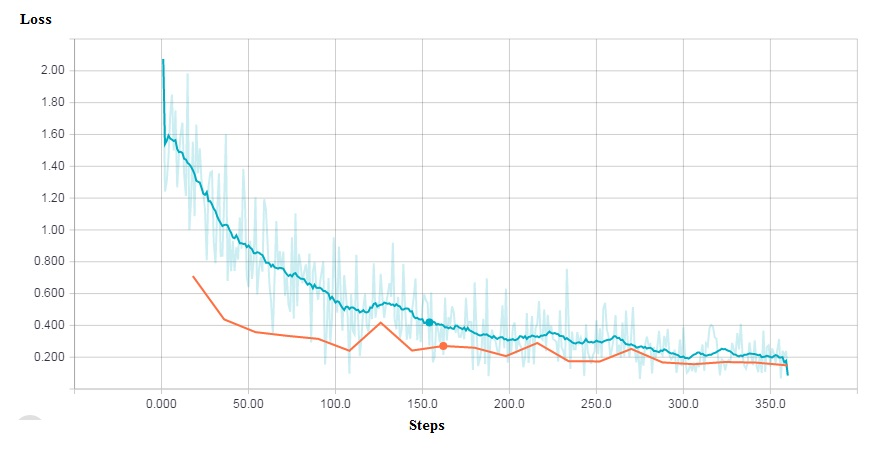
\includegraphics [width=\linewidth]{LossOverSteps.jpg}
\caption[\titlecap{Change in loss function over steps.}]{Change in loss function over steps (blue is training data, red is 10\% dev data).}
\label{fig:loss}
\end{figure*}

\begin{figure*}[tb]
\centering
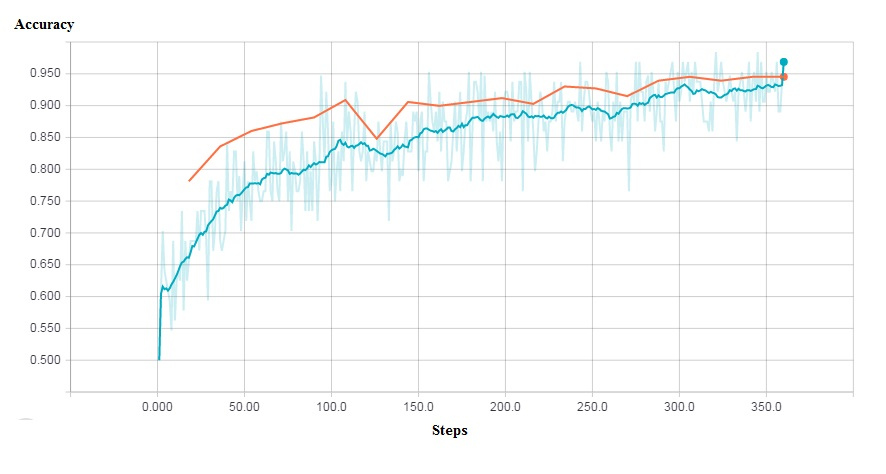
\includegraphics [width=\linewidth]{Accuracyoversteps.jpg}
\caption[\titlecap{Change in accuracy over steps.}]{Change in accuracy over steps (blue is training data, red is 10\% dev data).}
\label{fig:accuracy}
\end{figure*}

\subsection{Loss Function and Accuracy}


The loss is a measurement of the error our network makes, and our goal is to minimize it. The loss function for categorization problems is the cross-entropy loss.
$tf\cdot{nn}\cdot{softmax}\cdot{cross}\char`_entropy\char`_with\char`_logits$ is a function that calculates the cross-entropy loss for each class, given our scores and the correct input labels. We have then taken the mean of the losses. We could also use the sum, but that makes it harder to compare the loss across different batch sizes and train/dev data. Figure~\ref{fig:loss} shows the change cross-entropy loss over steps.

We also used an expression for the accuracy, which is a useful quantity to calculate the performance during training and testing. Change in accuracy over steps is shown in Figure~\ref{fig:accuracy}.

\subsection{Method Comparison}



We compared iGen with other state-of-the-art methods like Support Vector Machine (SVM)~\cite{cortes}, Naïve Bayes Classifier~\cite{nir}, and KNN (K-Nearest Neighbour)~\cite{liao1} classifier used for IOC sentence categorization. Three type of feature vector are used for each of the classifier described above. 10-fold cross validation technique is used to compare precision, recall and F-measure. Our comparative analysis is shown in Table~\ref{table:methodcompare}.

iGen outperformed other methods by generating IOCs with a precision of 95\% and a recall of 99\%, while among other SVM with tfidf as feature vector performed well with a precision and recall of 90\%.

Similarly, another approach iACE~\cite{liao} proposed by Liao gave promising result in extracting IOC with high accuracy. But iACE used around 5,283 terms as features which were manually gathered from the dataset. This implies that it will work very accurately on one dataset but may fail on sentences where different terminologies were used while writing the article. In case of iGen, features were not selected manually but features were selected by CNN automatically. This property makes iGen more adaptive towards any kind of data. 
 

\begin{table}[!tb]
	\centering
	\begin{tabular}{|c|c|c|c|}
		\hline
		\multicolumn{1}{|c|}{\textbf{Methods}} & \multicolumn{1}{c}{\textbf{Precision}} & \multicolumn{1}{|c|}{\textbf{Recall}} & \multicolumn{1}{|c|}{\textbf{F-measure}}\\
		\hline
		iGen & $\mathbf{95\%}$ & $\mathbf{99\%}$ & $\mathbf{97\%}$ \\
		\hline
		SVM \,\footnotemark[1] (Bag of words) & 89\% & 88\% & 88\% \\
		\hline
		SVM (tf\,\footnotemark[2]) &  90\% & 89\% & 89\% \\
		\hline
		SVM (tfidf\,\footnotemark[3]) &  90\% & 90\% & 90\% \\
		\hline
		Naive Bayes (Bag of words) & 81\% & 78\% & 79\% \\ % inserting body of the table
		\hline
		Naive Bayes (tf) &  83\% & 79\% & 81\% \\
		\hline
		Naive Bayes (tfidf) &  85\% & 83\% & 83\% \\
		\hline
		5-NN\,\footnotemark[4] (Bag of words) & 80\% & 80\% & 80\% \\ % inserting body of the table	
		\hline
		5-NN (tf) &  81\% & 81\% & 80\% \\
		\hline
		5-NN (tfidf) &  83\% & 82\% & 82\% \\[1ex] % [1ex] adds vertical space
		
		
		
		\hline
	\end{tabular}
	\caption[\titlecap{Comparative analysis with other methods}]{Results of our iGen models against other methods. $\mathbf{SVM}$ (Support Vector Machine), $\mathbf{NB}$ (Naive Bayes), and $\mathbf{5-NN}$ (5-Nearest Neighbours) classifiers were compared with feature vectors as bag of words (BOW), term frequency (tf), and term frequency - inverse document frequency (tfidf). }
	\label{table:methodcompare}
\end{table}


%\begin{table}[!tb]
%\caption{Results of our iGen models against other methods. $\mathbf{SVM}$ (Support Vector Machine), $\mathbf{NB}$ (Naive Bayes), and $\mathbf{5-NN}$ (5-Nearest Neighbours) classifiers were compared with feature vectors as bag of words (BOW), term frequency (tf), and term frequency - inverse document frequency (tfidf).  } % title of Table
%\centering % used for centering table
%\begin{tabular}{c c c c} % centered columns (4 columns)
%\hline\hline %inserts double horizontal lines
%Methods & Precision & Recall & F-measure \\ [0.5ex] % inserts table
%%heading
%\hline % inserts single horizontal line
%iGen & $\mathbf{95\%}$ & $\mathbf{99\%}$ & $\mathbf{97\%}$ \\
%SVM \,\footnotemark[1] (Bag of words) & 89\% & 88\% & 88\% \\ % inserting body of the table
%
%SVM (tf\,\footnotemark[2]) &  90\% & 89\% & 89\% \\
%SVM (tfidf\,\footnotemark[3]) &  90\% & 90\% & 90\% \\
%Naive Bayes (Bag of words) & 81\% & 78\% & 79\% \\ % inserting body of the table
%Naive Bayes (tf) &  83\% & 79\% & 81\% \\
%Naive Bayes (tfidf) &  85\% & 83\% & 83\% \\
%5-NN\,\footnotemark[4] (Bag of words) & 80\% & 80\% & 80\% \\ % inserting body of the table
%5-NN (tf) &  81\% & 81\% & 80\% \\
%5-NN (tfidf) &  83\% & 82\% & 82\% \\[1ex] % [1ex] adds vertical space
%
%\hline %inserts single line
%\end{tabular}
%\label{table:methodcompare} % is used to refer this table in the text
%\end{table}

\footnotetext[1]{SVM --- Support Vector Machine.}
\footnotetext[2]{tf --- Term Frequency.}
\footnotetext[3]{tfidf --- Term Frequency Inverse Document Frequency.}
\footnotetext[4]{5-NN --- 5-Nearest Neighbour}
\chapter{DISCUSSION AND FUTURE WORK} \label{chap:discussion}
Our experiments show that iGen not only fully automated the process of cyber threat intelligence collection but also generates deployable security rules from the data. With a large amount of IOCs automatically recovered from the wild and converted into a machine-readable form, these can be quickly and effectively utilized to counter emerging threats. For example, knowing the IP of C\&C server from APT report and then finding the email associated with IP address from malware report can help us find the actor behind the attack. This will enable the defender to disable or block the servers associated with that email to stop future attacks. On the other hand, our current design is still preliminary. Here, we discuss the limitations of iGen and potential follow-up research.

\subsection{Limitations}
Although iGen extracts IOC with high accuracy, precision and recall, but it's necessary to recognize our system limitations. First, iGen assumes that all the IOCs mentioned in the article are part of some sentence. But there is a possibility that some of them are present in images (e.g., command prompt screenshots) or tables inserted into the article. Second, even though iGen detects IOCs with high accuracy. iGen still introduces some false discoveries and misses some IOCs. These problems mostly arises due to abnormal ways of writing the report. Typos in articles or reports effects the performance of iGen. For example, if one forgets to place a space after the period, a sentence becomes held with the follow-up one, which could cause an error in IOC sentence classification. Further efforts are desirable to better address these issues.
\chapter{Conclusion}


\chapter{CONCLUSION} \label{chap:conclusion}

In this paper, we introduced --- CNN based iGen, a novel system for automatic extraction of IOCs from different sources of unstructured data. Our approach starts from collection of security data from diverse sources. Then, it cleans the data using advanced NLP techniques. CNN based IOC identification technique is found to be highly effective, immensely outperforming the top industry IOC analyzer tool in terms of accuracy, precision and recall. iGen generates ready-to-deploy rules from these IOCs that can be directly deployed on security infrastructure like NIDS etc.

iGen uses different sources for data to make fully automated cyber threat intelligence gathering more collaborative. iGen has collected around 1 million IOCs till now with a precision of 95\%, better than any state-of-art method. 

%-----------------------back matter
{\singlespace
% Making the references a "part" rather than a chapter gets it indented at
% level -1 according to the chart: top of page 4 of the document at
% ftp://tug.ctan.org/pub/tex-archive/macros/latex/contrib/tocloft/tocloft.pdf
\addcontentsline{toc}{part}{REFERENCES}
\bibliographystyle{asudis}
%\bibliographystyle{unsrt}
\bibliography{dis}}
\nocite{*}
\renewcommand{\chaptername}{APPENDIX}
\addtocontents{toc}{APPENDIX \par}
\appendix
\chapter{Raw Data}

\end{document}
